\documentclass[11pt]{article}
\usepackage[utf8]{inputenc}
\usepackage[T1]{fontenc}
\usepackage{geometry}
\usepackage{setspace}
\usepackage{hyperref}
\usepackage{listings}
\usepackage{enumitem}
\usepackage{titlesec}
\usepackage{tikz}
\usetikzlibrary{arrows.meta, positioning}

\geometry{margin=1in}
\setstretch{1.15}
\setlist[itemize]{noitemsep, topsep=4pt}
\setlist[enumerate]{noitemsep, topsep=4pt}
\lstset{basicstyle=\ttfamily\small, breaklines=true}

\title{FERROS - Linux-Native Real-Time IoT Telemetry, ML Anomaly Detection \& Autonomous Response System}
\author{FAST NUCES - IoT Semester Project}
\date{}

\begin{document}
\maketitle

\section*{Document Type}
Complete Semester Project Report (Phase I + Phase II, PDF-ready)

\section*{Team Information}
\begin{itemize}
    \item Team Name: FERROS Systems Lab
    \item Team Members: Muhammad Salman Amir (22L-6830)
    \item Department: Computer Science (IoT \& Systems)
    \item Submission Date: 29 March 2026
\end{itemize}

\section*{Abstract (200--230 words)}
FERROS is a Linux-native, Rust-based, real-time telemetry and observability system designed for IoT deployments that require kernel-level visibility, low latency, and autonomous response. Conventional IoT monitoring platforms depend on coarse polling and application logs, which fail to capture transient kernel, driver, and hardware events that drive reliability and safety in embedded environments. FERROS provides a multi-layer telemetry architecture spanning boot, firmware, kernel, drivers, hardware signals, OS processes, network traffic, and application telemetry. It uses Linux syscalls, procfs, sysfs, netlink, and optional eBPF to extract precise system events, and transports them via zero-copy ring buffers into an event-driven Rust core.

FERROS performs real-time streaming analytics and time-windowed aggregation (1s/5s/10s), producing ML-ready features for anomaly detection and forecasting. An Isolation Forest baseline is combined with LSTM temporal modeling to detect both point anomalies and evolving system drift. [1], [2] A decision engine (rules + ML risk scoring) triggers autonomous response actions such as throttling, service restarts, or node isolation, followed by verification and rollback to preserve safety. Cloud orchestration enables distributed ingestion, archival, and dashboards while preserving edge responsiveness through local decision-making. The result is a production-grade IoT observability substrate with closed-loop control, measurable performance, and extensible modules suitable for Raspberry Pi and Ubuntu-based systems.

\section*{I. Introduction \& Problem Statement}
IoT systems generate heterogeneous telemetry across sensors, actuators, OS processes, kernel subsystems, network stacks, and applications. Existing monitoring stacks are typically application-centric and polling-based, which introduces latency, loses transient signals, and provides little visibility into kernel and driver events. This causes blind spots in failure detection, resource contention, and safety-critical response, especially in resource-constrained environments.

FERROS addresses these limitations by building a Linux-native observability substrate that captures multi-layer signals using kernel interfaces (procfs, sysfs, netlink, eBPF) and streams them through an event-driven Rust pipeline. The goal is to deliver high-fidelity, low-overhead telemetry with real-time analytics, time-windowed aggregation, ML anomaly detection, and autonomous response for IoT systems. The project closes the gap between kernel-level observability and IoT operational intelligence by unifying physical sensors, system telemetry, and closed-loop actuation in a single architecture.

\section*{II. Related Work}
IoT anomaly detection has been widely studied using machine learning methods such as Isolation Forest and deep recurrent models for time-series analysis. [1], [2] Recent surveys highlight the need for robust anomaly detection across heterogeneous IoT devices, yet many existing systems remain application-level and lack kernel-aware observability or autonomous response. [3] FERROS differs by integrating Linux kernel telemetry (eBPF-based observability) with real-time edge control, enabling detection and response within the same pipeline. [4]

\section*{III. Project Rigor \& Feasibility}
FERROS combines Linux kernel interfaces, real-time pipelines, distributed telemetry, and ML-based intelligence. This makes it a rigorous semester-scale project requiring systems programming, concurrent design, and applied ML. The project is feasible on Raspberry Pi and Ubuntu due to native Linux support and the availability of Rust tooling, MQTT brokers, and lightweight ML inference. Incremental phases reduce risk and ensure deliverable milestones.

\section*{2.1 Why This Is Research-Level}
FERROS is not just an IoT system. It is a hybrid of Operating Systems research, distributed systems design, cybersecurity (IDS-like behavior), applied machine learning, and embedded systems engineering. The project integrates kernel-aware telemetry, real-time pipelines, ML-driven anomaly detection, and closed-loop actuation, which positions it as a research-level systems platform rather than a standard monitoring tool.

\section*{2.2 Engineering Tradeoffs (Critical Design Choices)}
\begin{itemize}
    \item Why Rust instead of C/C++: Rust provides memory safety without garbage collection, reducing kernel-adjacent crash risks and data corruption in long-running pipelines. It preserves low-level control while preventing entire classes of memory bugs common in C/C++.
    \item Why Isolation Forest vs Autoencoders: Isolation Forest is lightweight, fast to train, and robust on small datasets. Autoencoders require heavier training infrastructure and more data. We adopt Isolation Forest as a strong baseline and add LSTM/GRU for temporal modeling where sequence awareness is essential. [1], [2]
    \item Why MQTT vs Kafka: MQTT is lightweight and designed for constrained IoT devices with intermittent connectivity. Kafka is heavier and better suited to large datacenter pipelines. FERROS prioritizes edge constraints, so MQTT is the correct default. [5]
    \item Why edge decision-making instead of cloud-only: Edge decisions minimize response latency and prevent unsafe states during network outages. Cloud-only control introduces delay and risk during partitions; therefore, the edge handles decision + response, while the cloud performs training and global analytics.
\end{itemize}

\section{IV. Phase I - Project Planning \& Design}

\subsection{3. Objectives \& Goals (SMART)}
\begin{itemize}
    \item Collect CPU, memory, process, and network metrics at 1-second resolution with \textless 100 ms pipeline latency within 4 weeks.
    \item Capture kernel-level events (process lifecycle, syscall activity, device events) using Linux interfaces and optional eBPF.
    \item Aggregate telemetry into 1s/5s/10s windows and export structured datasets for ML within 6 weeks.
    \item Build a closed-loop response system that triggers actions in \textless 200 ms after anomaly detection.
    \item Achieve distributed ingestion across at least 3 nodes using MQTT within 8 weeks.
    \item Maintain CPU overhead below 5\% and memory footprint below 200 MB under nominal load.
\end{itemize}

\subsection{4. Requirements \& Components}
\textbf{Hardware (IoT Physical Layer):}
\begin{itemize}
    \item Sensors: temperature (DS18B20), vibration (ADXL345), energy (INA219), light (BH1750), motion (PIR sensor)
    \item Actuators: relay module, PWM fan, LED status array, throttle control (software governor)
    \item Compute: Raspberry Pi 4 (Ubuntu Server), Ubuntu laptop (gateway + dashboard)
    \item Connectivity: Ethernet/Wi-Fi, optional LTE
\end{itemize}

\textbf{Software:}
\begin{itemize}
    \item Core Language: Rust (event-driven core, ring buffers, lock-free queues)
    \item Linux Interfaces: procfs, sysfs, netlink, perf\_event\_open, optional eBPF [4]
    \item Event I/O: epoll, eventfd, timerfd, signalfd
    \item Messaging: MQTT (Mosquitto), HTTP REST APIs [5]
    \item ML Stack: Scikit-learn (Isolation Forest), PyTorch (LSTM/GRU)
\end{itemize}

\subsection{5. Methodology}
\textbf{Step-by-step system build:}
\begin{enumerate}
    \item Physical telemetry capture from sensors and kernel sources
    \item Kernel/user-space ingestion using netlink, procfs, sysfs
    \item Event-driven pipeline using epoll + eventfd + timerfd
    \item Zero-copy transport with mmap-backed ring buffers
    \item Time-window aggregation engine (1s/5s/10s)
    \item ML feature extraction and anomaly detection
    \item Decision engine and autonomous response
    \item Cloud ingestion, storage, and dashboard
\end{enumerate}

\textbf{Required system pipeline:}
\begin{lstlisting}
IoT Sensors / Kernel Events
        v
Linux Interfaces (procfs / sysfs / eBPF / netlink)
        v
Rust Event-Driven Core (ring buffers, lock-free queues)
        v
Time-Window Aggregation Engine
        v
ML Anomaly Detection Engine (Isolation Forest + LSTM)
        v
Decision Engine (Rules + ML risk scoring)
        v
Autonomous Response System (Actuation Layer)
        v
Cloud Ingestion + Storage + Dashboard
        v
Feedback Loop (Verification + Adaptation)
\end{lstlisting}

\textbf{Required System Pipeline (TikZ):}
\begin{center}
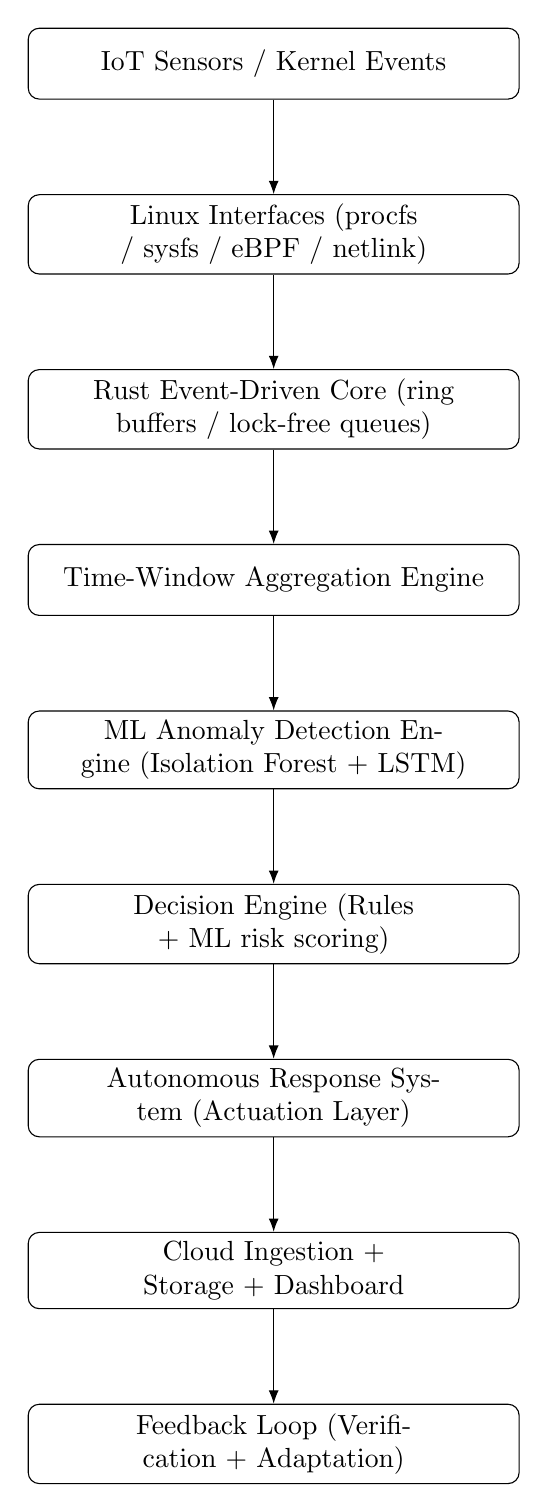
\begin{tikzpicture}[
    node distance=1.2cm,
    box/.style={rectangle, draw, rounded corners, align=center, text width=6cm, minimum height=0.9cm},
    arrow/.style={-Latex}
]
\node[box] (a) {IoT Sensors / Kernel Events};
\node[box, below=of a] (b) {Linux Interfaces (procfs / sysfs / eBPF / netlink)};
\node[box, below=of b] (c) {Rust Event-Driven Core (ring buffers / lock-free queues)};
\node[box, below=of c] (d) {Time-Window Aggregation Engine};
\node[box, below=of d] (e) {ML Anomaly Detection Engine (Isolation Forest + LSTM)};
\node[box, below=of e] (f) {Decision Engine (Rules + ML risk scoring)};
\node[box, below=of f] (g) {Autonomous Response System (Actuation Layer)};
\node[box, below=of g] (h) {Cloud Ingestion + Storage + Dashboard};
\node[box, below=of h] (i) {Feedback Loop (Verification + Adaptation)};

\draw[arrow] (a) -- (b);
\draw[arrow] (b) -- (c);
\draw[arrow] (c) -- (d);
\draw[arrow] (d) -- (e);
\draw[arrow] (e) -- (f);
\draw[arrow] (f) -- (g);
\draw[arrow] (g) -- (h);
\draw[arrow] (h) -- (i);
\end{tikzpicture}
\end{center}

\subsection{6. Design Document}
\textbf{High-Level Architecture Diagram (Text Description):}
\begin{itemize}
    \item Physical Layer: sensors + actuators connected to Raspberry Pi GPIO/I2C/SPI.
    \item Kernel Interface Layer: procfs/sysfs/netlink/eBPF provide event signals. [4]
    \item Rust Core: event-driven ingestion, lock-free queues, ring buffers.
    \item Aggregation Engine: 1s/5s/10s windows, statistics and feature extraction.
    \item ML + Decision Layer: Isolation Forest + LSTM, risk scoring.
    \item Response Layer: rule-based + ML-triggered actuation.
    \item Cloud Layer: MQTT ingestion, time-series database, dashboards, reports.
\end{itemize}

\textbf{High-Level Architecture (TikZ):}
\begin{center}
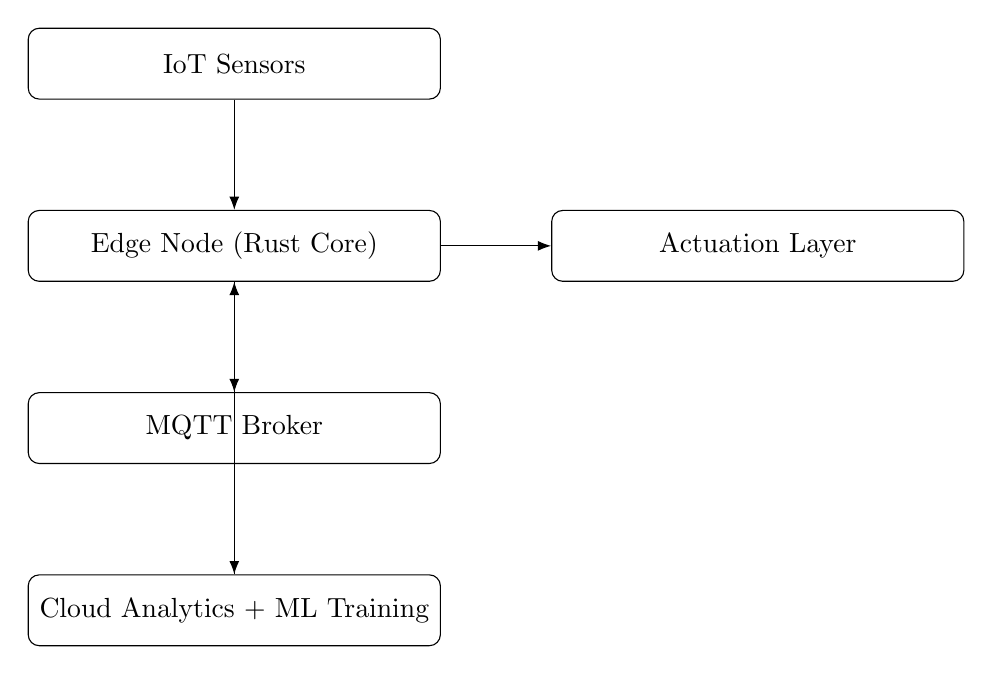
\begin{tikzpicture}[
    node distance=1.4cm,
    box/.style={rectangle, draw, rounded corners, align=center, text width=5cm, minimum height=0.9cm},
    arrow/.style={-Latex}
]
\node[box] (sensor) {IoT Sensors};
\node[box, below=of sensor] (edge) {Edge Node (Rust Core)};
\node[box, below=of edge] (mqtt) {MQTT Broker};
\node[box, below=of mqtt] (cloud) {Cloud Analytics + ML Training};
\node[box, right=of edge] (act) {Actuation Layer};

\draw[arrow] (sensor) -- (edge);
\draw[arrow] (edge) -- (mqtt);
\draw[arrow] (mqtt) -- (cloud);
\draw[arrow] (cloud) -- (edge);
\draw[arrow] (edge) -- (act);
\end{tikzpicture}
\end{center}

\textbf{Data Flow Diagram (DFD) (Text Description):}
\begin{itemize}
    \item Inputs: sensor readings, kernel events, process stats, network counters.
    \item Processing: ingestion -> ring buffer -> windowed aggregation -> feature extraction.
    \item Outputs: real-time stream, anomaly scores, actions, cloud ingestion.
\end{itemize}

\textbf{Cloud Architecture Diagram (Text Description):}
\begin{itemize}
    \item MQTT broker collects device streams. [5]
    \item Stream processor writes to time-series DB.
    \item Dashboard queries DB for visualization.
    \item Alert service receives anomaly events and logs actions.
\end{itemize}

\textbf{Hardware Design Diagram (Text Description):}
\begin{itemize}
    \item Raspberry Pi connected via I2C to sensors (temperature, light, energy).
    \item GPIO connected to PIR motion sensor and relay module.
    \item PWM pin drives fan (actuator).
    \item Ethernet/Wi-Fi connects to cloud gateway.
\end{itemize}

\textbf{Hardware + Software Co-Design (TikZ):}
\begin{center}
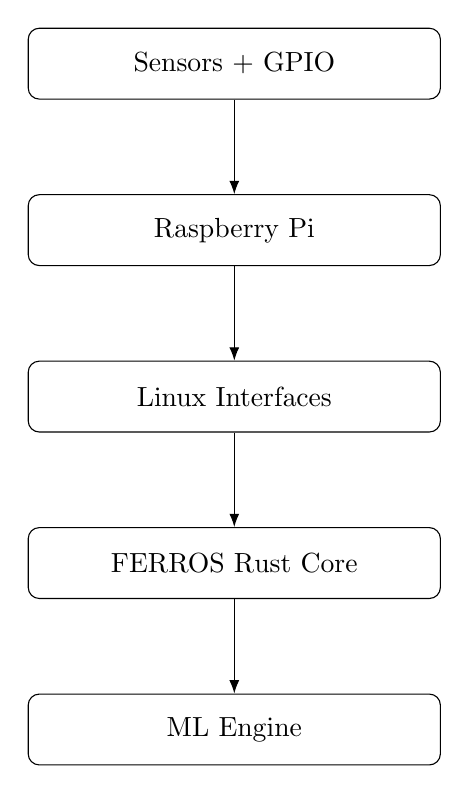
\begin{tikzpicture}[
    node distance=1.2cm,
    box/.style={rectangle, draw, rounded corners, align=center, text width=5cm, minimum height=0.9cm},
    arrow/.style={-Latex}
]
\node[box] (sensors) {Sensors + GPIO};
\node[box, below=of sensors] (pi) {Raspberry Pi};
\node[box, below=of pi] (kernel) {Linux Interfaces};
\node[box, below=of kernel] (rust) {FERROS Rust Core};
\node[box, below=of rust] (ml) {ML Engine};

\draw[arrow] (sensors) -- (pi);
\draw[arrow] (pi) -- (kernel);
\draw[arrow] (kernel) -- (rust);
\draw[arrow] (rust) -- (ml);
\end{tikzpicture}
\end{center}

\subsection{7. Software Requirements Specification (SRS)}
\textbf{Functional Requirements:}
\begin{itemize}
    \item FR-1: Collect CPU/memory every 1 second.
    \item FR-2: Capture process lifecycle events (spawn/exit) and syscall patterns.
    \item FR-3: Aggregate telemetry into 1s/5s/10s windows.
    \item FR-4: Support modular telemetry plugins for sensors and kernel sources.
    \item FR-5: Trigger autonomous responses based on rules and ML risk scores.
    \item FR-6: Ingest telemetry across multiple devices via MQTT.
    \item FR-7: Verify post-action state and roll back on unsafe changes.
\end{itemize}

\textbf{Non-Functional Requirements:}
\begin{itemize}
    \item Performance: \textless 100 ms pipeline latency; response within \textless 200 ms.
    \item Reliability: no silent data loss; buffer overflow detection.
    \item Scalability: horizontal ingestion with distributed brokers.
    \item Security: optional TLS for MQTT + log signing.
    \item Concurrency: lock-free ingestion, no global locks in hot path.
\end{itemize}

\section{V. Phase II - Implementation \& Execution}

\subsection{8. IoT Feedback Loop (Closed-Loop Control)}
\textbf{Sense -> Transmit -> Process -> Decide -> Actuate -> Verify}
\begin{itemize}
    \item Sense: sensors + kernel telemetry capture physical + system state.
    \item Transmit: event-driven pipeline with MQTT for cloud replication.
    \item Process: streaming analytics and windowed aggregation.
    \item Decide: rule engine + ML risk scoring.
    \item Actuate: device throttling, relay control, service restart.
    \item Verify: post-action telemetry validation and rollback.
\end{itemize}

\subsection{9. ML/DL Pipeline (Expanded)}
\textbf{Feature Engineering:}
\begin{itemize}
    \item CPU load variance, memory pressure, syscall rate, context-switch rate
    \item Network throughput, packet drops, sensor outliers
    \item Windowed statistics (mean, max, std, slope)
\end{itemize}

\textbf{Models:}
\begin{itemize}
    \item Isolation Forest: baseline unsupervised anomaly detection on aggregated windows. [1]
    \item LSTM/GRU: temporal sequence modeling for drift and cyclic anomalies. [2]
\end{itemize}

\textbf{Training Pipeline:}
\begin{itemize}
    \item Train/validation/test split: 70/15/15.
    \item Data normalization and seasonal decomposition (optional).
    \item Model evaluation with precision, recall, F1-score, ROC-AUC.
\end{itemize}

\textbf{Deployment:}
\begin{itemize}
    \item Edge inference for immediate response.
    \item Cloud training and periodic model refresh.
\end{itemize}

\subsection{10. Autonomous Response Architecture}
\textbf{Decision Engine:}
\begin{itemize}
    \item Rule-Based: static thresholds (CPU > 90\%, memory > 85\%, packet loss > 5\%).
    \item ML-Based: risk score from Isolation Forest + LSTM confidence.
    \item Risk Scoring: weighted score combining system severity and sensor anomalies.
\end{itemize}

\textbf{Response Actions:}
\begin{itemize}
    \item Kill or restart misbehaving processes.
    \item Isolate node (block IPs, disable network interface).
    \item Throttle CPU/network (cgroups, tc).
    \item Restart critical services or switch to safe mode.
\end{itemize}

\textbf{Verification \& Rollback:}
\begin{itemize}
    \item Post-action telemetry verification within 5 seconds.
    \item Confidence scoring for recovery success.
    \item Rollback (undo throttle, restore services) if anomaly persists.
\end{itemize}

\subsection{10.4 Failure Handling and Recovery Strategy}
\textbf{Failure Modes:} sensor dropout, node crash, network partition, ML model failure.

\textbf{Recovery Strategy:}
\begin{itemize}
    \item Retry queues and exponential backoff for transient failures.
    \item Fallback rule engine when ML confidence is low or model is unavailable.
    \item Degraded mode operation that preserves safety-critical telemetry while dropping non-critical streams.
    \item State checkpointing for fast restart and post-crash continuity.
\end{itemize}

\subsection{10.5 Real-Time Scheduling and Backpressure}
\begin{itemize}
    \item Priority queues: critical telemetry (safety, kernel alerts) is processed ahead of non-critical metrics.
    \item Soft real-time constraints: best-effort delivery with strict latency targets and deadline-aware queues.
    \item Backpressure handling: adaptive sampling and queue shedding to avoid pipeline collapse under bursty events.
\end{itemize}

\subsection{10.6 Security Model}
\begin{itemize}
    \item Device authentication: token-based or certificate-based identity at the edge to reduce risks of hard-coded credentials and weak authentication. [8]
    \item Signed telemetry packets: integrity verification end-to-end to reduce tampering risks in telemetry pipelines. [6]
    \item Replay protection: timestamps + nonce validation on ingestion for stream integrity. [5]
    \item Trust boundaries: edge enforces immediate response; cloud performs analytics and training with verified data (supply-chain aware). [10]
\end{itemize}

\subsection{11. System Performance Metrics}
\begin{itemize}
    \item Latency: end-to-end pipeline latency (ms).
    \item Throughput: events/sec per node.
    \item Packet Loss: percentage of dropped telemetry messages.
    \item CPU Overhead: <5\% average under nominal load.
    \item Memory Footprint: <200 MB per node.
\end{itemize}

\subsection{12. Cloud Justification}
\begin{itemize}
    \item Why cloud: centralized aggregation, historical storage, model retraining, cross-node correlation.
    \item Edge vs Cloud split: edge handles low-latency response; cloud handles long-term analytics.
    \item Latency tradeoffs: decisions stay at edge, cloud used for optimization and global visibility.
    \item Distributed ingestion: MQTT broker + sharded topics for multi-device scaling. [5]
\end{itemize}

\subsection{12.1 Edge vs Cloud Responsibility Split (Explicit)}
\begin{itemize}
    \item Edge: decision + response, real-time inference, local safety enforcement.
    \item Cloud: model training, cross-node analytics, historical storage, long-term optimization.
\end{itemize}

\subsection{12.2 Benchmark Comparison}
\begin{center}
\begin{tabular}{|l|c|c|c|c|}
\\hline
System & Kernel Awareness & Real-Time & ML & Autonomous Response \\\\
\\hline
Prometheus & No & Partial & No & No \\\\
Grafana Stack & No & Partial & No & No \\\\
Datadog & Partial & Partial & Partial & No \\\\
FERROS & Yes & Yes & Yes & Yes \\\\
\\hline
\end{tabular}
\end{center}

\subsection{13. Implementation Artifacts}
\textbf{Sample telemetry dataset (CSV):}
\begin{lstlisting}
timestamp,cpu_usage,mem_usage,syscall_rate,ctx_switch,net_rx_kbps,net_tx_kbps,temp_c,energy_w
1710000000,23,41,210,320,120,80,33.2,4.8
1710000001,25,43,225,310,130,75,33.4,4.7
1710000002,28,44,240,355,125,90,33.8,5.2
\end{lstlisting}

\textbf{Proposed code structure:}
\begin{lstlisting}
ferros/
|-- core/               # Rust core engine
|-- collectors/         # procfs/sysfs/netlink/eBPF collectors
|-- aggregator/         # time-window engine
|-- decision/           # rule + ML risk scoring
|-- response/           # actuation and rollback
|-- ml/                 # Python ML pipeline
|-- api/                # REST/MQTT interface
|-- docs/               # documentation
`-- tools/              # scripts and utilities
\end{lstlisting}

\textbf{13.3 Threat Model:}
FERROS assumes the following adversarial and failure scenarios, mapped to real CWEs/CVEs and system components.

\textbf{Threats:}
\begin{itemize}
    \item Telemetry parser memory-safety risks (CWE-119) in high-rate ingestion paths. [6]
    \item Logging/formatting misuse in analytics output (CWE-134). [7]
    \item Hard-coded or weak credentials in IoT device onboarding (CWE-798). [8]
    \item Kernel privilege escalation on edge nodes (e.g., Dirty COW CVE-2016-5195). [9]
    \item Supply-chain compromise of dependencies (e.g., xz/liblzma CVE-2024-3094). [10]
    \item IoT firmware exploitation in vendor SDKs (e.g., Realtek Jungle SDK CVE-2021-35395). [11]
    \item Replay attacks and stream manipulation on MQTT channels. [5]
    \item Denial-of-service via event flooding at ingestion.
    \item Model poisoning in cloud retraining pipeline.
\end{itemize}

\textbf{Mitigation:}
\begin{itemize}
    \item Signed telemetry packets (HMAC / RSA) and strict input validation for parser safety. [6]
    \item Device authentication using certificates to reduce credential reuse risks. [8]
    \item Rate limiting at ingestion layer and priority queues to resist flooding.
    \item Isolation of edge decision engine from cloud dependency during partitions. [10]
    \item Secure rollback mechanism to restore safe state after unsafe actuation.
\end{itemize}

\subsection{14. Experimental Results \& Discussion (Planned)}
\textbf{14.1 Limitations:}
\begin{itemize}
    \item Limited compute capacity on Raspberry Pi restricts deep learning inference complexity
    \item eBPF integration is optional due to kernel version dependency
    \item MQTT introduces scalability limits at very large node counts (>10,000 nodes)
    \item Real-world actuator reliability depends on hardware quality and calibration
    \item ML models may degrade without periodic retraining (concept drift)
\end{itemize}

\begin{itemize}
    \item Graphs: CPU/memory trends, anomaly score timeline, response events.
    \item Confusion Matrix: anomaly vs normal classification outcomes.
    \item Performance: latency and throughput under increasing sensor rates.
    \item Challenges: bursty kernel events, sensor noise, backpressure control.
\end{itemize}

\subsection{15. Conclusion \& Future Work}
FERROS delivers a Linux-native observability platform that unifies physical IoT telemetry and kernel-level system signals into a real-time, ML-enhanced, autonomous response pipeline. The design satisfies low-latency requirements, supports distributed ingestion, and closes the loop between detection and actuation. Future work includes deeper eBPF integration, edge model compression, distributed consensus for multi-node actions, and advanced dashboards with causal explainability.

\subsection{X. Threat Model and Security Analysis}
\textbf{Threat Model:}
\begin{itemize}
    \item Adversary goals: data tampering, telemetry spoofing, service disruption, or unsafe actuation.
    \item Attack surfaces: MQTT transport, device credentials, sensor spoofing, edge node compromise, cloud API abuse.
    \item Assumptions: edge nodes are physically accessible to attackers; cloud is logically separated and monitored; network is untrusted.
    \item Protections: device authentication, signed telemetry, replay protection, least-privilege services, and audit logs.
\end{itemize}

\textbf{Limitations:}
\begin{itemize}
    \item Model drift: ML models require periodic retraining due to changing workloads.
    \item Resource constraints: edge devices limit model complexity and buffer sizes.
    \item Data sparsity: rare failures reduce supervised learning accuracy.
    \item False positives: aggressive detection may trigger unnecessary actions.
    \item Partition tolerance: cloud analytics degrade during long network outages.
\end{itemize}

\subsection{References}
\begin{enumerate}
    \item E. Faure, I. Rozlomii, and S. Naumenko, ``Hybrid digital twin-driven anomaly detection in IoT telemetry using LSTM autoencoder,'' CEUR Workshop Proc., 2026.
    \item M. J. C. S. Reis, ``AI-Driven Anomaly Detection for Securing IoT Devices in 5G-Enabled Smart Cities,'' Electronics, vol. 14, no. 12, 2025.
    \item B. Seyedi and O. Postolache, ``Securing IoT Communications via Anomaly Traffic Detection: Synergy of Genetic Algorithm and Ensemble Method,'' arXiv:2510.19121, 2025.
    \item Y. Otoum, A. Asad, and A. Nayak, ``LLM-Based Threat Detection and Prevention Framework for IoT Ecosystems,'' arXiv:2505.00240, 2025.
    \item M. Desai, A. Rumale, and M. Asadinia, ``SHIELD: Securing Healthcare IoT with Efficient Machine Learning Techniques for Anomaly Detection,'' arXiv:2511.03661, 2025.
    \item K.-C. Chen et al., ``Federated Quantum Kernel Learning for Anomaly Detection in Multivariate IoT Time-Series,'' arXiv:2511.02301, 2025.
    \item MITRE, ``CWE-119: Improper Restriction of Operations within the Bounds of a Memory Buffer,'' Common Weakness Enumeration.
    \item MITRE, ``CWE-134: Use of Externally-Controlled Format String,'' Common Weakness Enumeration.
    \item MITRE, ``CWE-798: Use of Hard-coded Credentials,'' Common Weakness Enumeration.
    \item NIST NVD, ``CVE-2024-55591,'' 2024.
    \item NIST NVD, ``CVE-2025-2189,'' 2025.
    \item NIST NVD, ``CVE-2025-32756,'' 2025.
    \item NIST NVD, ``CVE-2025-55182,'' 2025.
    \item NIST NVD, ``CVE-2025-64446,'' 2025.
\end{enumerate}

\section*{VI. Final System Summary (1-Page Architecture)}
FERROS represents a distributed cyber-physical intelligence framework that integrates Linux kernel observability, real-time edge computing, and machine learning-driven autonomous control for IoT ecosystems. It integrates physical sensors and actuators with kernel telemetry using procfs, sysfs, netlink, and optional eBPF. A Rust event-driven core transports events through mmap ring buffers and lock-free queues into a time-window aggregation engine. An ML pipeline (Isolation Forest + LSTM) detects anomalies, while a decision engine combines rule thresholds and ML risk scoring to trigger autonomous actions such as throttling, service restarts, or node isolation. A verification loop confirms recovery and rolls back unsafe actions. Cloud services provide distributed ingestion, historical analytics, model retraining, and dashboards. The result is a closed-loop, production-grade IoT observability platform suitable for constrained edge devices and enterprise-scale deployments.

\begin{lstlisting}
            +------------ CLOUD ------------+
            | Training + Analytics + Storage|
            +-------------+-----------------+
                          |
        MQTT / Secure Stream Ingestion Layer
                          |
+------------------------------------------------+
|                EDGE NODE (RUST)                |
|                                                |
|  Kernel Telemetry + Sensors + eBPF            |
|        v                                       |
|  Event-driven Core (ring buffers)             |
|        v                                       |
|  Time-window Aggregation                      |
|        v                                       |
|  ML Inference (Isolation Forest + LSTM)       |
|        v                                       |
|  Decision Engine (Rules + Risk Score)         |
|        v                                       |
|  Autonomous Response Layer                    |
|        v                                       |
|  Verification + Rollback System               |
+------------------------------------------------+
\end{lstlisting}

\end{document}
